\section{Introdução}
A pobreza, segundo \citeauthor{gomide2003transporte} \citeyear{gomide2003transporte}, não é simplesmente a falta de renda para suprir as necessidades básicas, mas também envolve à privação de acesso aos serviços essenciais, tais como educação, saúde, transporte coletivo e aos direitos sociais básicos, como acesso ao trabalho, moradia e seguridade social. Portanto, além da renda e PIB per capita, os indicadores de acesso aos serviços e direitos sociais básicos apresentam análises relevantes sobre o conceito.
    
Para \cite{rolnik2002possivel}  a contraposição existente entre uma minoria qualificada e uma maioria em condições precárias está quase sempre relacionada a situação de exclusão territorial, dividindo assim a cidade entre uma porção legal, rica e influente, e uma ilegal, pobre e precária, sendo esta privada de oportunidade de trabalho, cultura ou lazer. Esses espaços, por vezes chamado periferia, podem ser definidos por “espaços socialmente homogêneos, esquecidos pelas políticas estatais e localizados tipicamente nas extremidades da área metropolitana”. \cite{vasconcellos2016mobilidade}
    
Existem diversas visões sobre as causas para esse padrão de urbanização no Brasil: o mercado de trabalho, a estrutura social, a dinâmica imobiliária para produção de moradias e as políticas estatais.  \cite{vasconcellos2016mobilidade}.

Nesse sentido, é importante que se faça uma análise da pobreza pela esfera espacial, relacionando políticas públicas de mobilidade criadas pelo Estado com a segregação da periferia, focando na Região Metropolitana de São Paulo. Claramente, as políticas públicas possuem limites e não se pode dizer que elas são as únicas causadoras da segregação e exclusão territorial, porém é importante perceber como essas políticas, ao longo da história, ampliaram as dimensões desses problemas. \cite{rolnik2002possivel}. Dessa forma, a fim de realizar as análises citadas, o presente trabalho usará a Região Metropolitana de São Paulo como objeto de estudos.
	
Na cidade de São Paulo, pode-se perceber que o direcionamento das políticas públicas sempre favoreceu o desenvolvimento do transporte individual, diferentemente das relacionadas ao transporte coletivo, que se caracterizam pelo "esforço mínimo", sendo apenas suficientes para realizar o transporte das pessoas até seus locais de trabalho, com qualidade e acessibilidade grandemente prejudicadas \cite{vasconcellos2016mobilidade}. Além disso, segundo \citeauthor{diamond2005colapso} \citeyear{diamond2005colapso} em seu livro “Colapso”, o uso do carro e a promoção de políticas que favoreciam o transporte individual em detrimento do coletivo deixaram o desenvolvimento de sistemas de transporte público, que suprissem as necessidades da população, sobretudo da periferia, fortemente prejudicado.
	
No Brasil, as políticas públicas de subsídio dadas ao transporte coletivo e ao individual diferem em oito vezes \cite{vasconcellos2012transporte}, ou seja, para cada R\$8,00 de subsídio dado ao transporte, apenas R\$1,00 vai para o coletivo. Essa diferença se contrapõe ao uso do transporte público, que nos grandes centros urbanos, 64\% das viagens motorizadas são feitas por ônibus e metrô \cite{ipea2011emissoes}.

Ainda segundo dados da prefeitura de São Paulo, a frota de ônibus urbano se manteve estável desde 2003. O gráfico da figura \ref{fig:frota_onibus} retirado do site do governo de São Paulo em 31 de maio de 2021, mostra a constância do número de ônibus.
    
\begin{figure}[!htbp]
	\centering
 	\caption{Número de ônibus da frota da SPTRANS}
	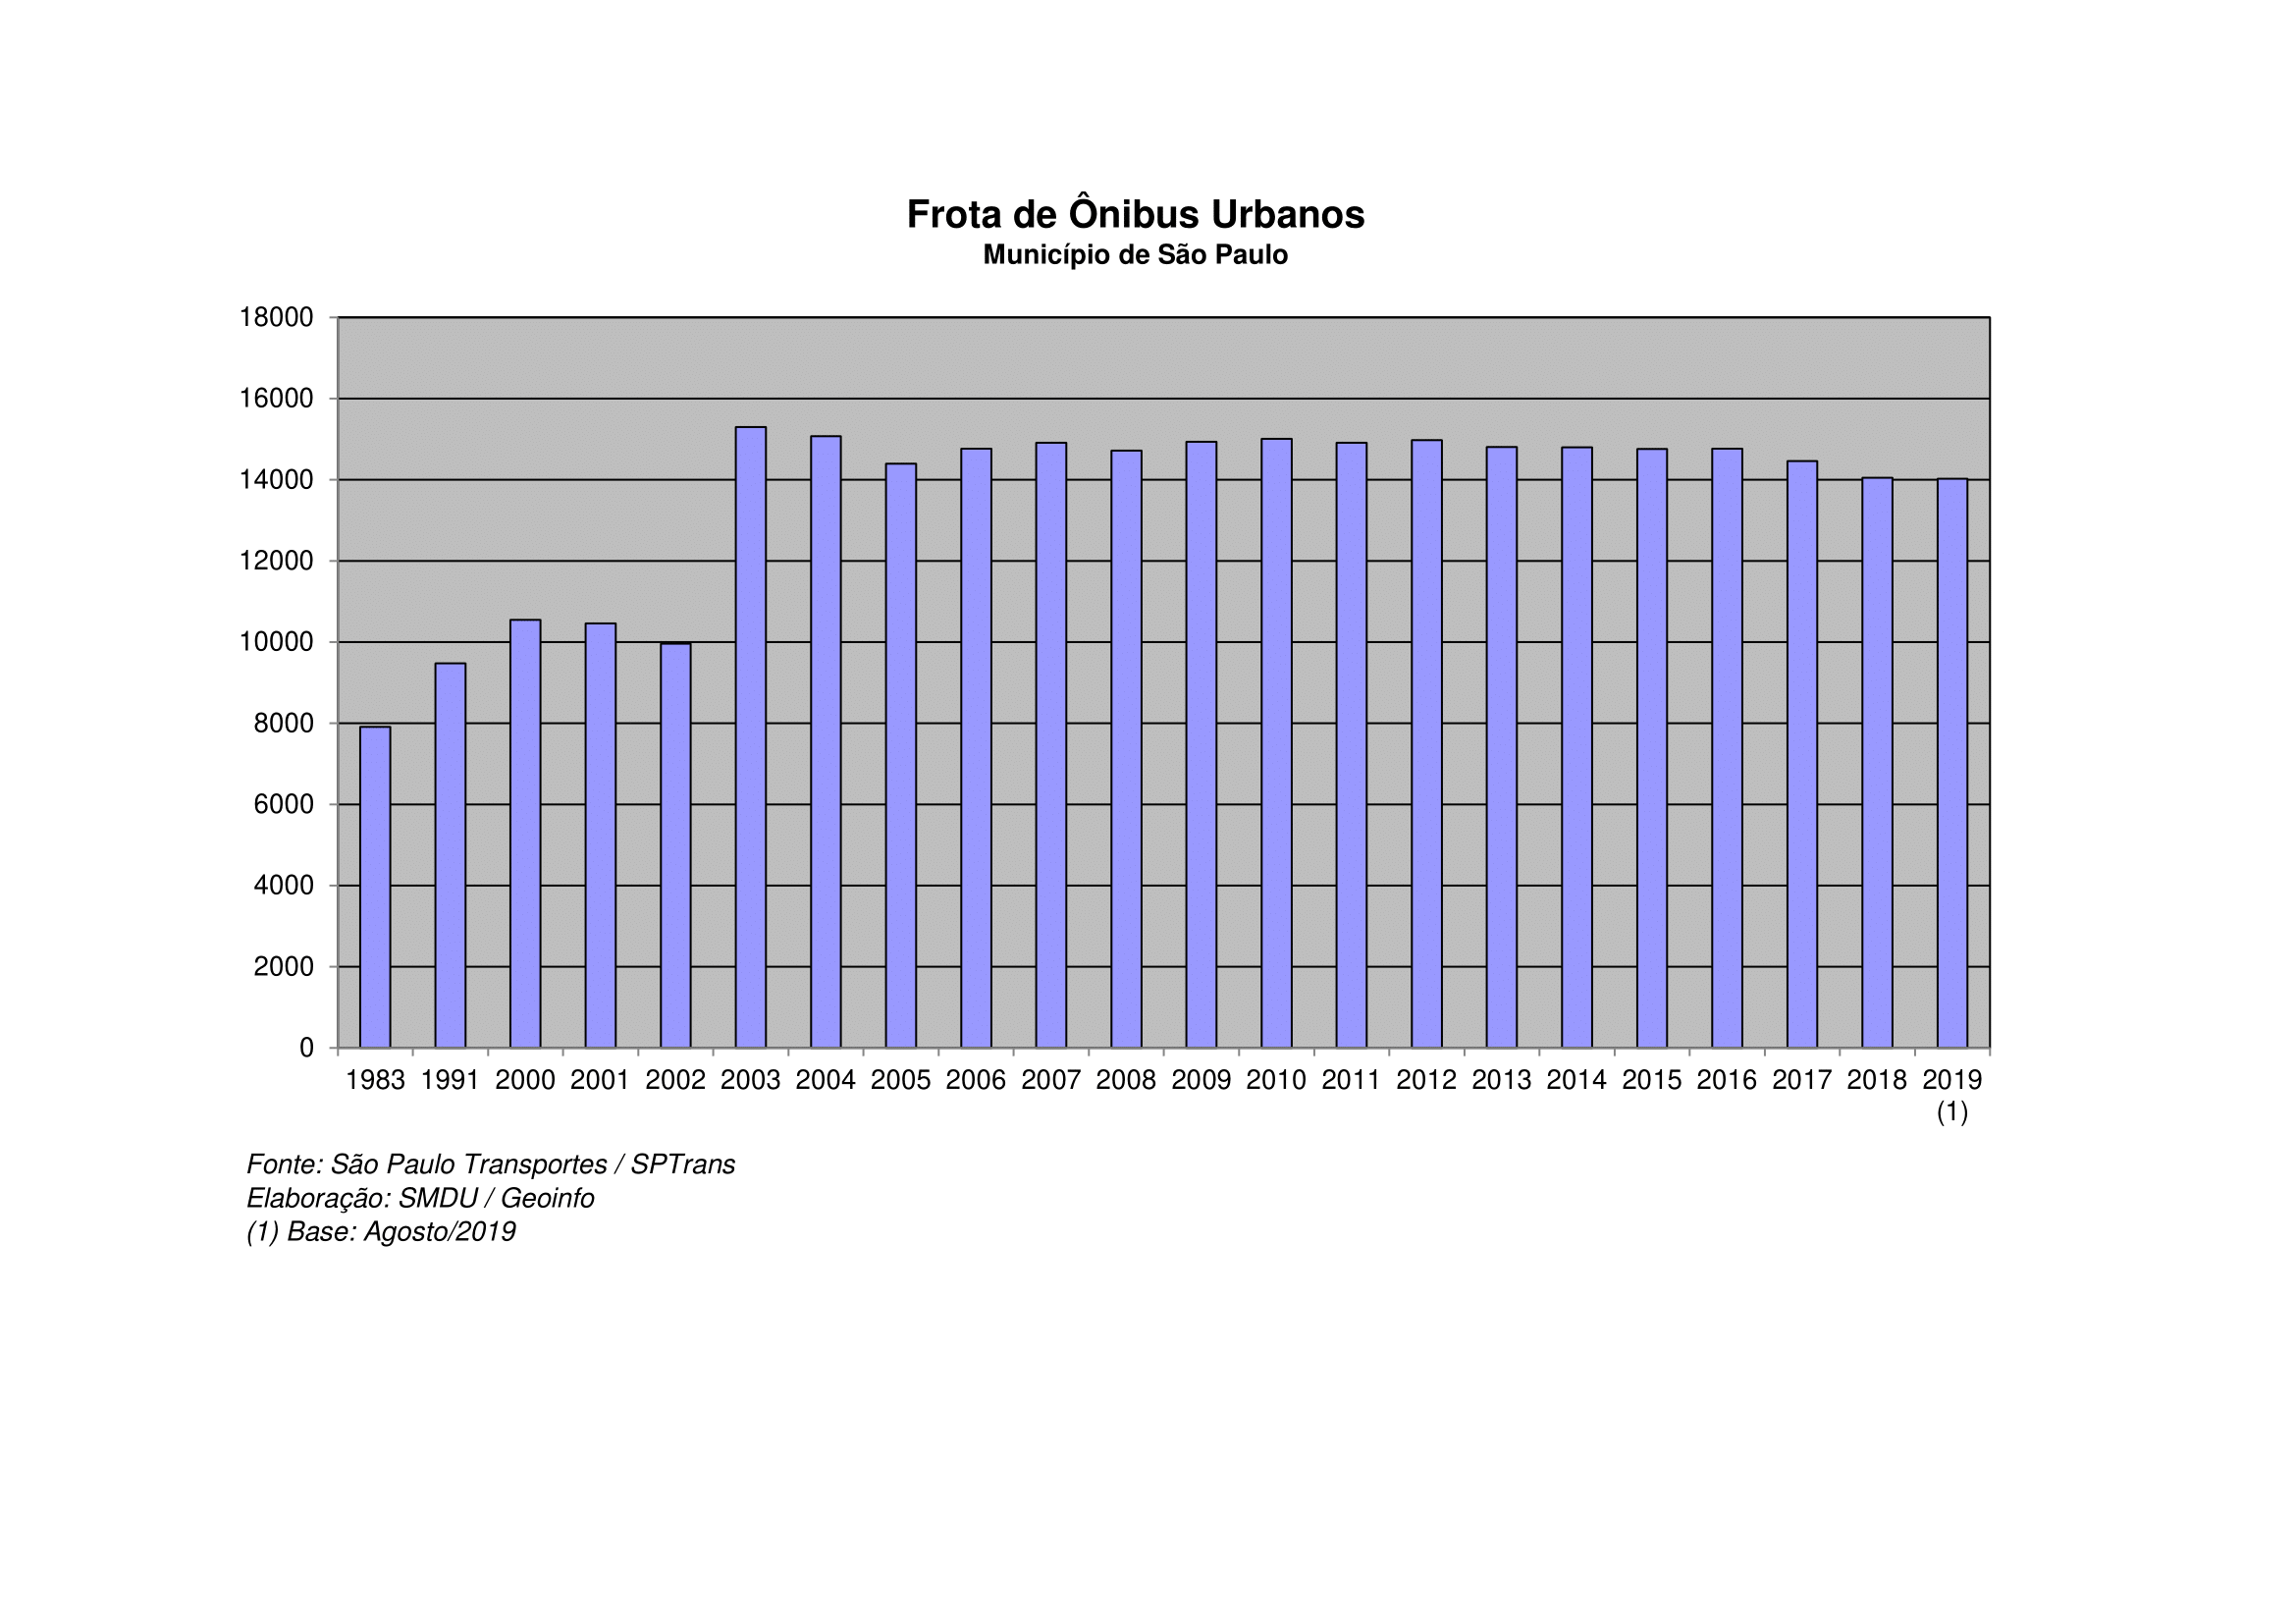
\includegraphics[scale=0.18]{introducao/frota_de_onibus_urbanos.png}
	\begin{flushleft}
	    {\footnotesize Fonte: \cite{graficoOnibus}}
	\end{flushleft}
	\label{fig:frota_onibus}
\end{figure}

No mesmo espaço de tempo, a frota de veículos quase dobrou, como mostra o gráfico da figura \ref{fig:veiculos_detranSP} de veículos cadastrados no Detran de São Paulo, acessado no dia 30 de maio de 2021.

\begin{figure}[!htbp]
	\centering
 	\caption{Número de veículos registrados no Detran SP}
	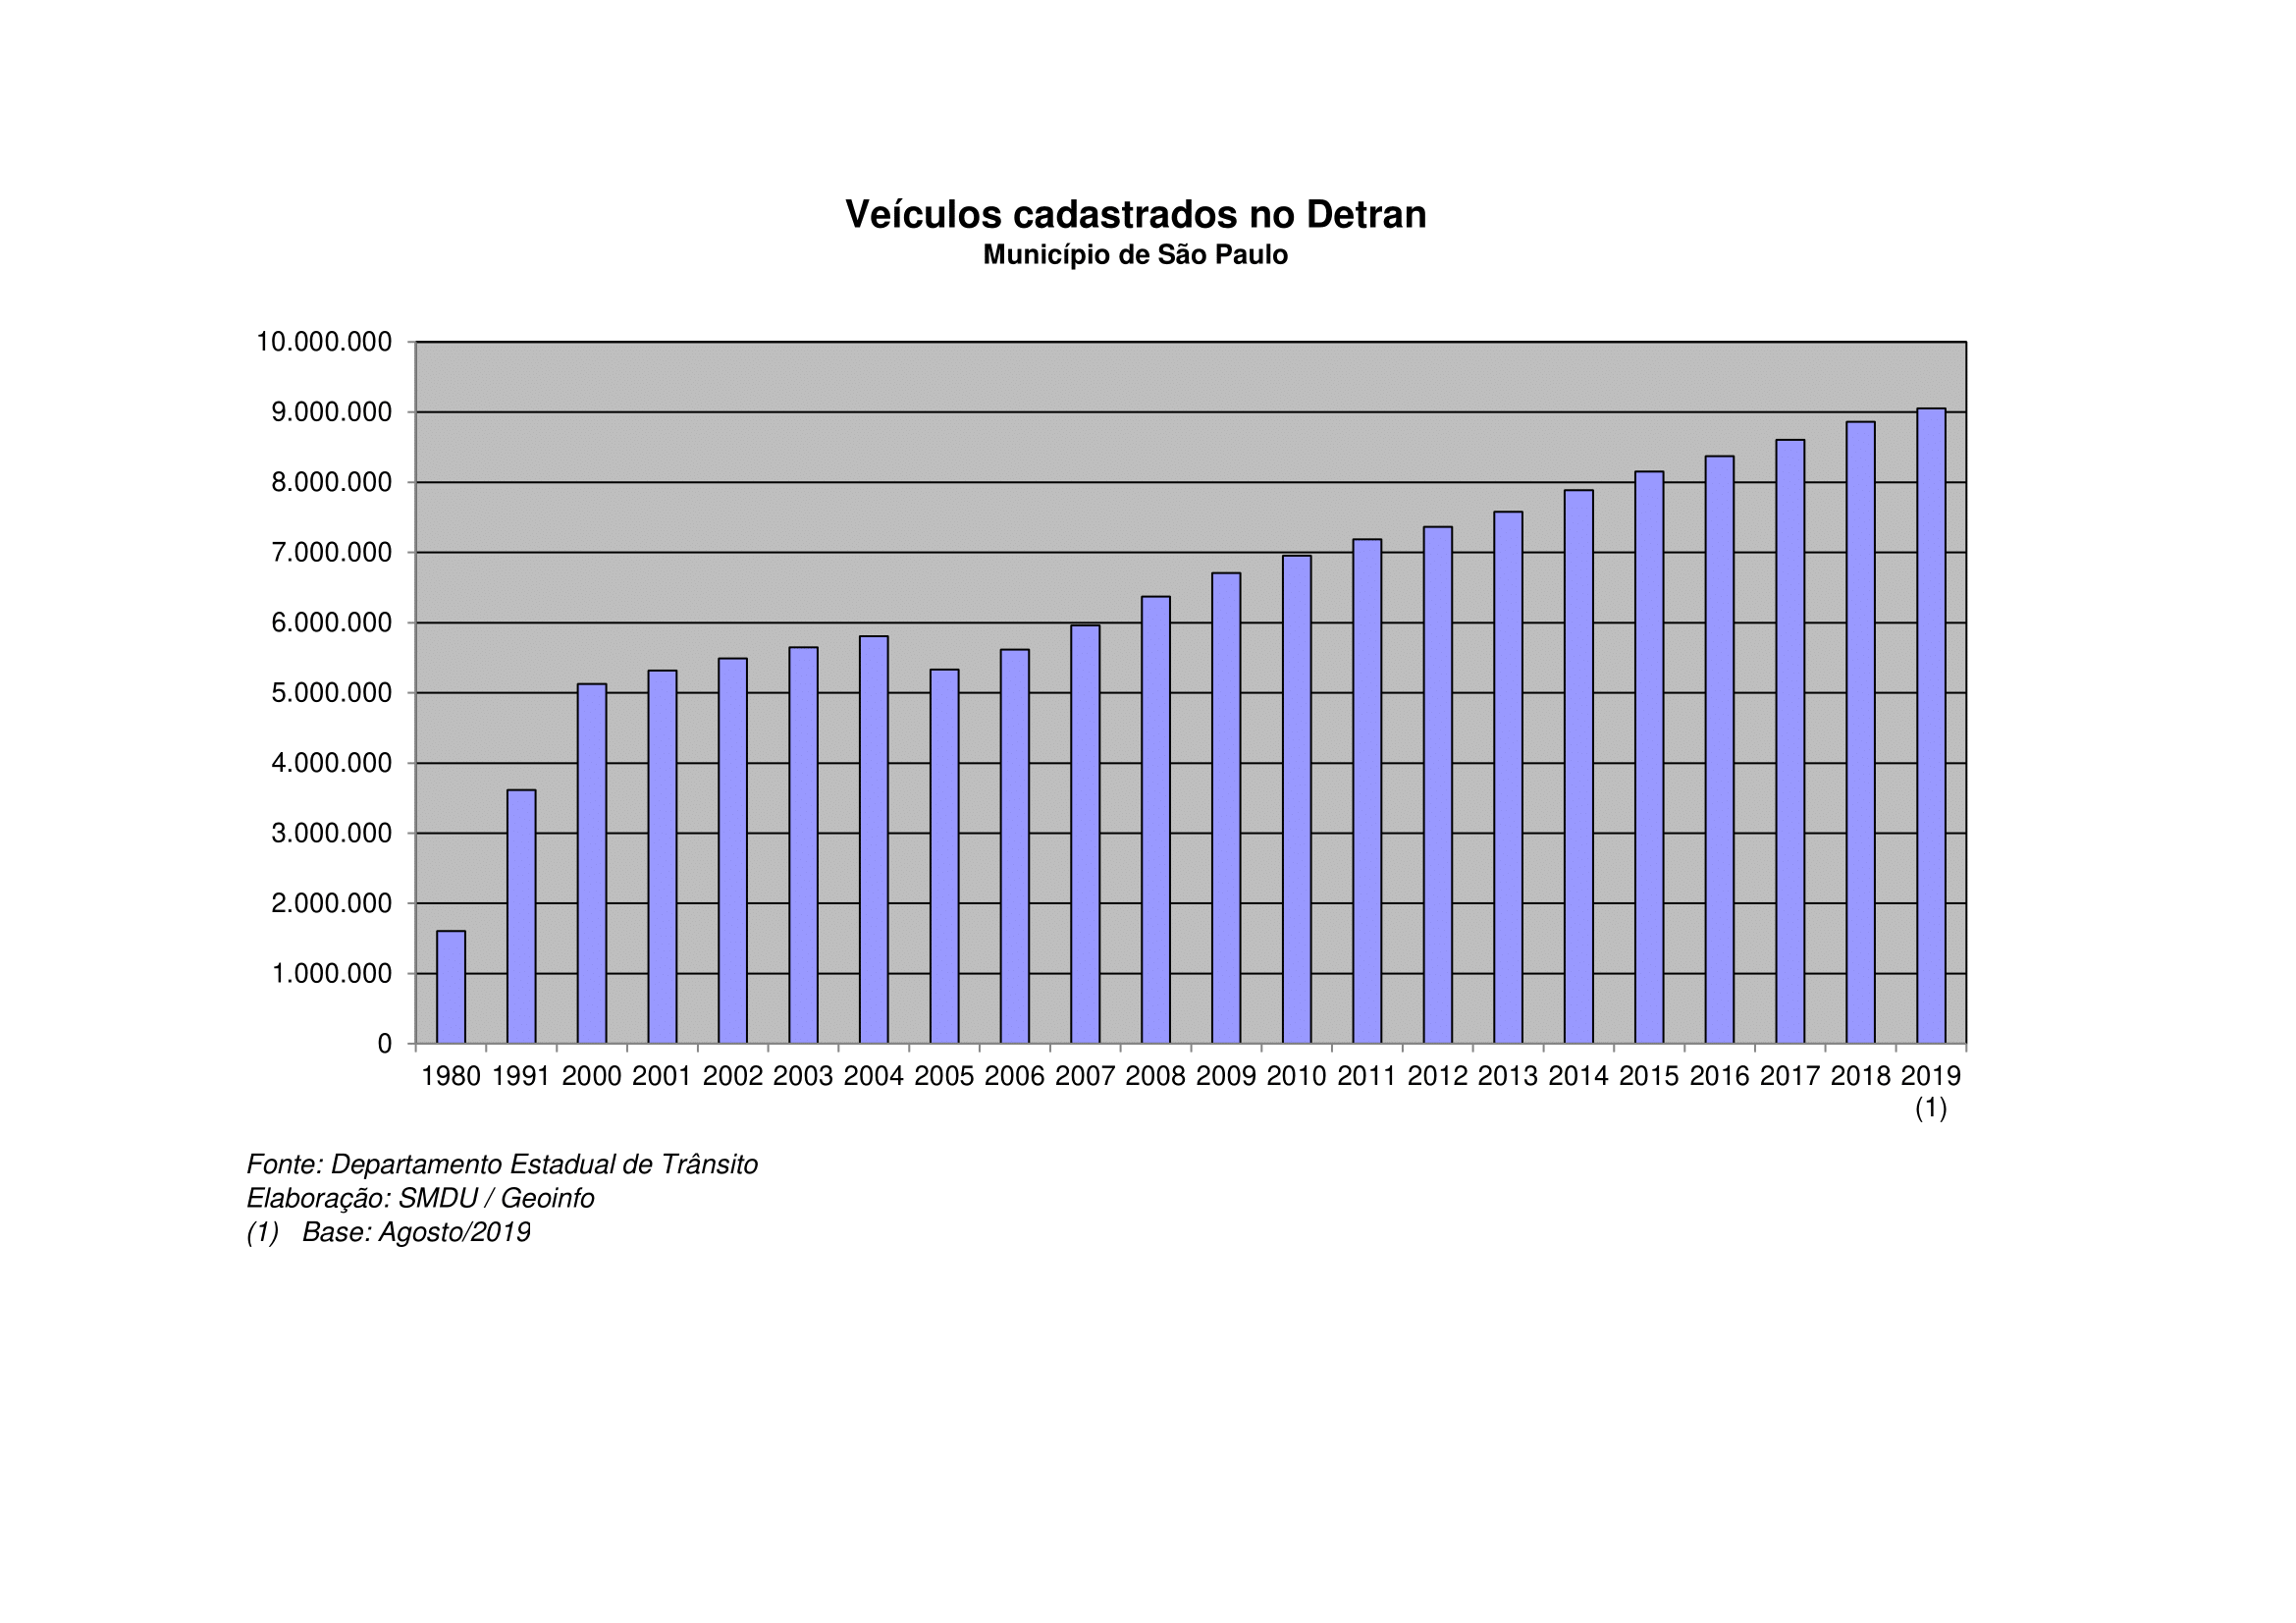
\includegraphics[scale=0.18]{introducao/veiculos.png}
	\begin{flushleft}
	    {\footnotesize Fonte: \cite{graficoVeiculos}}
	\end{flushleft}
	\label{fig:veiculos_detranSP}
\end{figure}

A diferença entre a constância da frota de ônibus e o crescimento do número de carros na cidade de São Paulo evidencia a disparidade de investimentos entre os transportes, aumentando o uso de carros e deixando estagnado o transporte coletivo, prejudicando, assim, o acesso das periferias a esse serviço.
	
Segundo \citeauthor{gomide2003transporte} \citeyear{gomide2003transporte}, o acesso a um transporte coletivo, eficiente e de qualidade é fundamental para a garantia da Constituição Federal, uma construção social que expressa os direitos fundamentais e universais do cidadão, na qual está incluso o transporte coletivo urbano \cite{constituicao} (Constituição Federal, artigo 30, inciso V). Assim, considerando o papel do contrato social que é a Constituição, sem o acesso aos serviços públicos essenciais, como o citado acima, os cidadãos estariam prejudicados no desenvolvimento de suas capacidades, no exercício de seus direitos e no ato de equiparar oportunidades com outras pessoas. 

Por fim, na pesquisa proposta, ao analisar a pobreza pela esfera espacial, focando na distribuição do transporte coletivo, serão entendidas as causas da segregação socioespacial e seu impacto na população periférica naquilo que se refere ao transporte, à pobreza e ao mercado de trabalho.